

\documentclass{acm_proc_article-sp}


\usepackage{graphicx}
\usepackage{listing}
\usepackage{listings} \lstset{basicstyle=\tiny,numbers=none, breaklines=true, numberstyle=\tiny, numbersep=5pt,firstnumber=last,language=XML,escapeinside={(*@}{@*)} }  

% *** CITATION PACKAGES ***
%
\usepackage{cite}
\usepackage{url}
%\usepackage[scaled=point85]{luximono}
\hyphenation{op-tical net-works semi-conduc-tor name-space}

\begin{document}

\title{VIENNA Add-In \\ Visualizing Inter-ENterprise Network Architectures}


%Do not change this number
\numberofauthors{2}


\author{
% You can go ahead and credit any number of authors here,
% e.g. one 'row of three' or two rows (consisting of one row of three
% and a second row of one, two or three).
%
% The command \alignauthor (no curly braces needed) should
% precede each author name, affiliation/snail-mail address and
% e-mail address. Additionally, tag each line of
% affiliation/address with \affaddr, and tag the
% e-mail address with \email.
%
% 1st. author
\alignauthor
Christian Huemer, Philipp Liegl, Thomas Motal, Rainer Schuster, Marco Zapletal \\
       \affaddr{Vienna University of Technology}\\
       \affaddr{Favoritenstrasse 9-11/188}\\
       \affaddr{1040 Vienna, Austria}\\
       \email{\{firstname.lastname\}@tuwien.ac.at}       
\alignauthor
Christian Eis, Martina Hiesinger, Fabian Kromer, Robert Kromer, Andreas Kuntner, Christian Pichler, Michael Strommer\\
       \affaddr{Research Studios Austria}\\
       \affaddr{Thurngasse 8/3/20}\\
       \affaddr{1090 Vienna, Austria}\\
       \email{\{firstname.lastname\}@researchstudio.at}       
% 2nd. author
%\alignauthor
%Christian Pichler\\
%       \affaddr{Research Studios Austria}\\
%       \affaddr{Thurngasse 8/3/20}\\
%       \affaddr{1090 Vienna, Austria}\\
%       \email{cpichler@researchstudio.at}
}

\date{28 April 2009}

\maketitle
\begin{abstract}

%What is the problem
The definition of concise and interoperable business documents has become one of the key issues in today's electronic business transactions. 
In this paper, we present our tool VIENNA Add-In supporting a business document modeler in creating Core Component compliant business document models using the Unified Modeling Language (UML). The core components standard defines reusable building blocks for constructing business documents and is maintained by UN/CEFACT (United Nations Center for Trade Facilitation and Electronic Business). Our tool provides a set of powerful features for core components such as model validation, semi-automatic generation of model artifacts, and generation of fully compliant XML Schema definitions from a conceptual model representation. Thereby, the VIENNA Add-In helps to shorten development cycles and reduces errors in designing business documents. The overall goal of our tool-based approach for inter-organizational processes is the generation of deployment artifacts for IT systems from conceptual models.


\end{abstract}
% A category with the (minimum) three required fields
\category{H.4}{Information Systems Applications}{Miscellaneous}
\terms{Business document modeling, conceptual modeling, XML schema generation}

\section{Introduction}
Before two business partners can engage in an automated Business-to-Business (B2B) interaction two agreements have to be made. First, the process choreography has to be specified, i.e., the exact exchange order of the different business documents. Second, the business information being exchanged in the electronic transaction must be specified, i.e., the business document definition. In a joint effort between the Vienna University of Technology\footnote{http://www.tuwien.ac.at/} and the Research Studios Austria, Studio Inter-Organisational Systems\footnote{http://ios.researchstudio.at/}, we have developed the VIENNA Add-In \cite{man:VIENNAAddIn}. The Add-In is built on top of the UML modeling tool Enterprise Architect (EA) from Sparx Systems. %\footnote{http://www.sparxsystems.com.au}.
\begin{figure}[htbp]
 \centering
   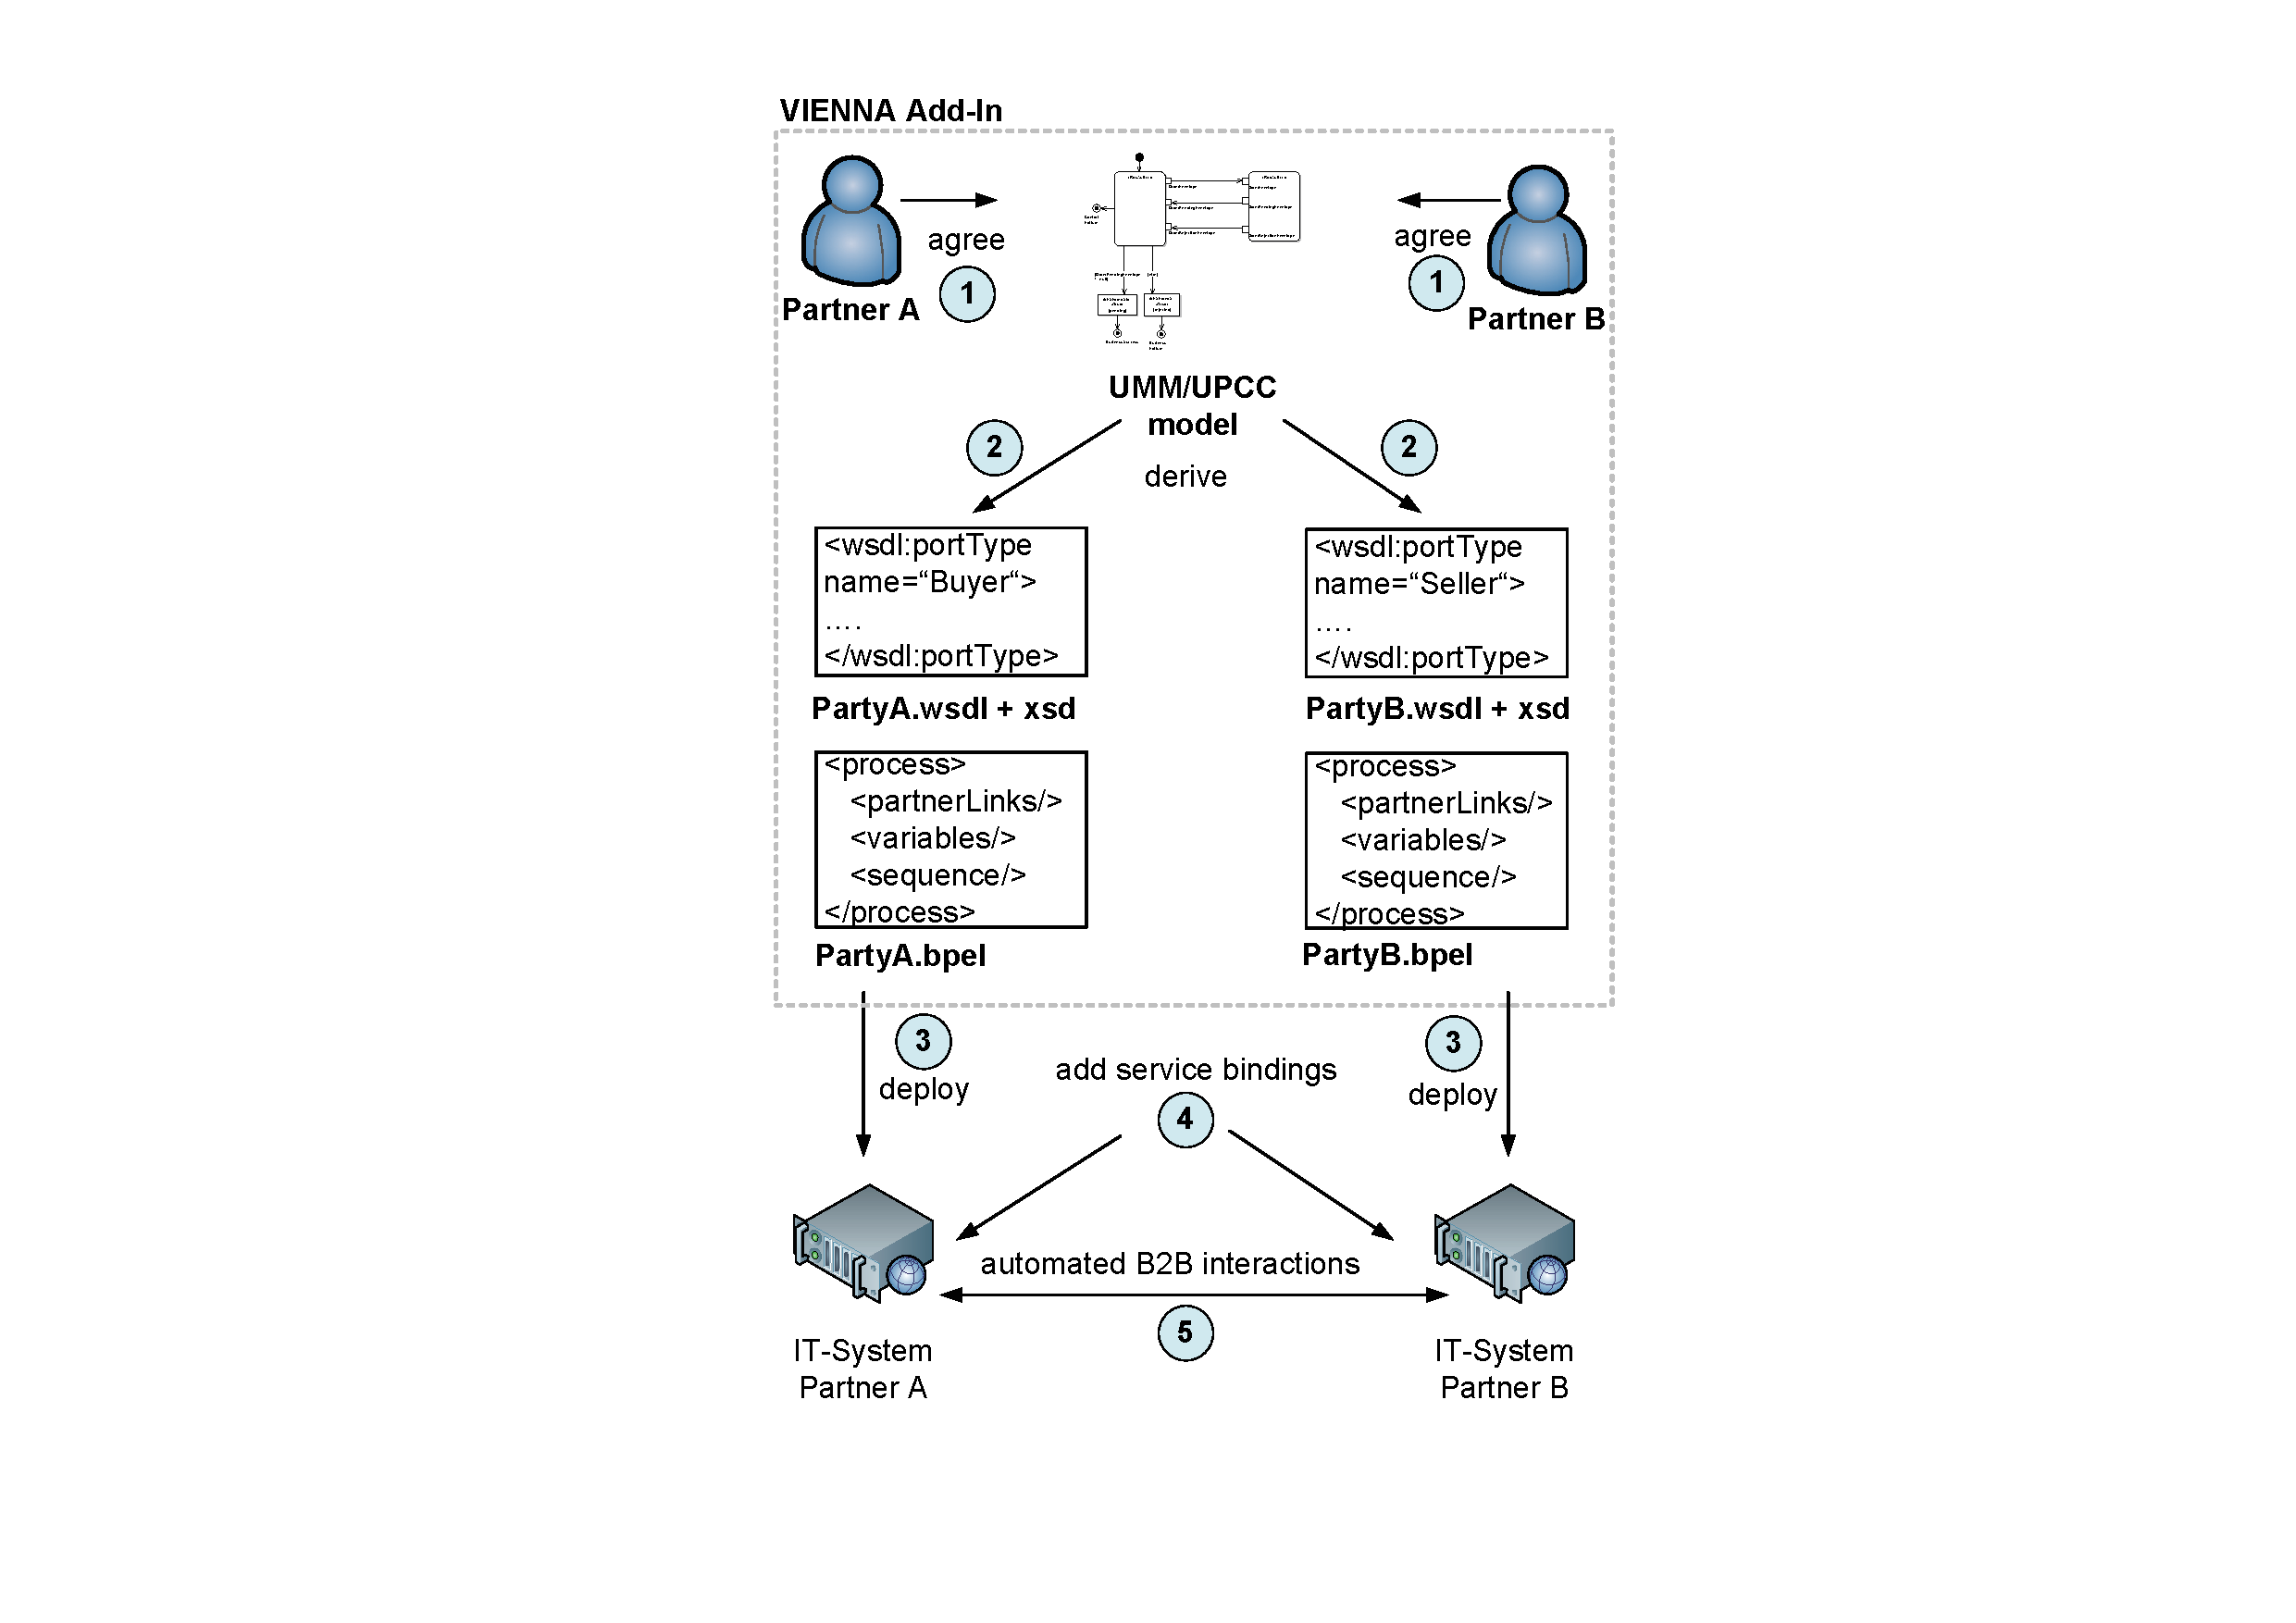
\includegraphics[width=0.32\textwidth]{figures/addinoverview.pdf}
 \caption{VIENNA Add-In overview}
 \label{fig:viennaaddinoverview}
\end{figure}
The VIENNA Add-In currently supports both, business choreography definitions and business document definitions. For the former the supported technology is UN/CEFACT's Modeling Methodology (UMM) \cite{man:umm2} and for the latter the UML Profile for UN/CEFACT's Core Components (UPCC) \cite{man:upcc}. \\Figure \ref{fig:viennaaddinoverview} gives a brief overview of the main approach pursued by the VIENNA Add-In. Two business partners willing to engage in an electronic collaboration first agree on a common UMM model specifying the business choreography and a common UPCC model specifying the exchanged business information (see (1) in Figure \ref{fig:viennaaddinoverview}). Both models are specified on a conceptual level using the Unified Modeling Language (UML). In a consecutive step the commonly agreed upon process and information model is used to derive deployment artifacts for the IT systems (2). Interface definitions and the exchanged information are reflected using WSDL and XML Schema artifacts. The local choreography definitions are reflected using Business Process Execution Language (BPEL) artifacts. Eventually the generated artifacts can be deployed to Business Service Interfaces (3). After adding service bindings (4) automatic B2B interactions are feasible (5). Thus, the business modeler is provided with a model driven approach for the definition of deployment artifacts for service oriented systems. Since the deployment artifacts for both business partners are derived from a common conceptual model, the business document definitions and process choreography definitions on both sides match. \\In our tool demonstration we will in particular focus on the business document specific features. The following three sections outline three of the core features of the VIENNA Add-In.

%: the definition of a UML Profile for Core Components, the semi-automatic generation of model artifacts, and the generation of XML Schema from conceptual business document models.

\section{UML Profile Definition}
%In order to support the modeling of UMM and UPCC within EA we utilized a so-called Model Driven Generation (MDG) technology. An MDG technology is a set of collected resources, such as UML profiles, UML patterns, and code templates, bundled into an XML file. 
Within Enterprise Architect users may extend the standard UML modeling features through utilizing so-called Model Driven Generation (MDG) technologies which are an EA specific extension mechanism. An MDG technology is a set of collected resources, such as UML profiles, UML patterns, and code templates, bundled into an XML file. We created MDG technologies for UMM and UPCC in order to support business process modeling and business document modeling in Enterprise Architect. Both MDG technology files are stored online\footnote{UMM: http://www.umm-dev.org/ea/umm2.xml\\UPCC:\; http://www.umm-dev.org/ea/upcc3.xml}. After successful configuration of EA these MDG technologies will be loaded dynamically during every EA startup. Dynamic loading provides a suitable solution in order to keep the technology automatically up-to-date to the most recent version. \\Additionally, we added proprietary features which are supported by EA, such as toolbox and diagram profiles, model templates, and quicklinks. The first two features support the use of custom element and diagram types in order to provide a development environment, which is shaped to the specifics of UMM and UPCC. \textit{Quick Links} are an additional feature, providing a context driven creation of new elements and relationships i.e. for a given model artifact allowed element associations are offered to the user. Subsequently the modeler may choose a suggested association and the association together with an optional new target element is automatically drawn.

\section{Semi-automatic artifact generation}

Having the necessary MDG technologies available in EA allows business document modeling on a conceptual level. The typical approach to model business documents involves three steps. First, different artifacts including enumeration types (ENUMs), primitive types (PRIMs), core data types (CDTs), and aggregate core components (ACCs) are modeled on the core component level. All artifacts modeled on the core component level represent domain-independent, re-usable, building blocks for business document modeling. Second, domain-specific artifacts, including business data types (BDTs) and aggregate business information entitites (ABIEs) are created on the business information entity level. The artifacts on the business information entity level are created through derivation by restriction from the artifacts on the core components level. \\ Especially deriving artifacts on the business information entity level involves simple but repetitive modeling tasks. Therefore, we implemented a set of wizards supporting the user in performing complex modeling tasks. At the moment, these features include a wizard for creating the default library structure as specified in the UPCC, a wizard for importing standard CC libraries published by UN/CEFACT, a wizard for creating and editing ABIEs, as well as a wizard for creating BDTs, and a wizard guiding the user through the process of generating XML Schema artifacts representing the business documents modeled. The generation of XML Schema artifacts is described in more detail in the following. 

\section{XML Schema generation}
In order to use the CCTS models composed with UPCC in a real world business process we provide the VIENNA Add-In with an XML Schema generator. The serialization of the XML Schema files is driven by the general Naming and Design Rules provided by UN/CEFACT \cite{CEFACT:NDR}. These Naming and Design Rules constitute a mapping between the conceptual model of CCTS and the XML Schema language. Thus, it is ensured that CCTS models conforming to these rules are interchangeable across platforms and applications. For every business document to be serialized a set of XML Schema files is created, reflecting the library structure of a standard UPCC model. For example, for an assembled business document in a document library (DOCLibrary), the libraries on the business information entity level (BIELibrary and BDTLibrary) are serialized into separate files as well. Following the specification in \cite{CEFACT:NDR} element annotations containing meaningful documentation are generated from the tagged values of the conceptual model as well. 

Until now the VIENNA Add-In supports the generation of XML schemas conforming to CCTS. However, it is desirable to have schema generators for other languages and other syntax, too. The support of new document models that are not based on CCTS mostly involves the manual mapping from a domain model to CCTS. Automation techniques such as matching may be considered as well. Currently, we also work on the implementation of generators for business process deployment artifacts such as BPEL files.


%2. outlook what should be supported

%\begin{enumerate}
%\item \emph{Serialize CCTS model.} This use case may most likely occur after modeling an arbitrary business document from scratch. The serialization of the XML Schema is driven by the general Naming and Design Rules provided by the UN/CEFACT \cite{CEFACT:NDR}. By doing so we ensure that CCTS models conforming to these rules are interchangeable across platforms and applications. 
%\item \emph{Serialize some model.} This use case is triggered at the end of step two during the transformation of say document model $M_A$ into document model $M_B$. The serialization of the XML Schema of model $M_B$ must adhere to the custom naming and design rules of the original document model on which the mapping from $M_B$ to CCTS $M_P$ was defined.  The generated schema will in most cases only cover a subset of the original model $M_B$, otherwise the transformation becomes obsolete.
%\item \emph{Serialize subset of some model.} After a particular subsetting of model $M_A$ to model $M_{A'}$  the generation of the schema follows specific naming and design rules as explained in the previous subtask. Furthermore, it has to be ensured that model $M_{A'}$ is strictly a subset of $M_A$ and does not contain any extensions. Otherwise instances $o_{A'}$ conforming to $M_{A'}$ will no longer be conforming to $M_A$ leading to further interoperability problems.
%\end{enumerate}
%Finally, in support of the schema generation use case, as well as the document subsetting use case, the Add-In provides functionality to serialize CCTS models as XML schema documents, according to the UN/CEFACT Naming and Design Rules. Generation of other XML schema documents, adhering to some arbitrary naming and design rules, is currently being worked on, as well as the use of Map Force mapping definitions for document transformations and round-trip engineering.





\bibliographystyle{abbrv}
\bibliography{references}  
\end{document}
